\documentclass[12pt]{article}
\usepackage{hyperref}
\usepackage{graphicx}
\usepackage{parskip}
\usepackage{float}
\usepackage{amsmath}

\hypersetup{
    colorlinks,
    citecolor=black,
    filecolor=black,
    linkcolor=black,
    urlcolor=black
}

\title{PEU 356 Assignment 1}
\author{Mohamed Hussien El-Deeb (201900052)}
\date{\today}

\begin{document}

\maketitle
\tableofcontents

\section{3.10.1}

\[
    xy = u, x^2 - y^2 = v, z = z
\]

\subsection{a}

\(u\) curves are \(\frac{n}{x}\) asymptotes, \(u=0\) is xz-plane, repeated for all values of \(z\).

\[
    (x, \frac{u_i}{x}, z)
\]

\(v\) curves are x shaped for \(v=0\), horizontal hyperbola for \(v>0\), vertical hyperbola for \(v<0\), repeated for all values of \(z\).

\[
    (x, \pm\sqrt{x^2 - v_i}, z)
\]

\(z\) curves are planes parallel to xy-plane.


\[
    (x, y, z_i)
\]

\subsection{b}

\begin{figure}[H]
    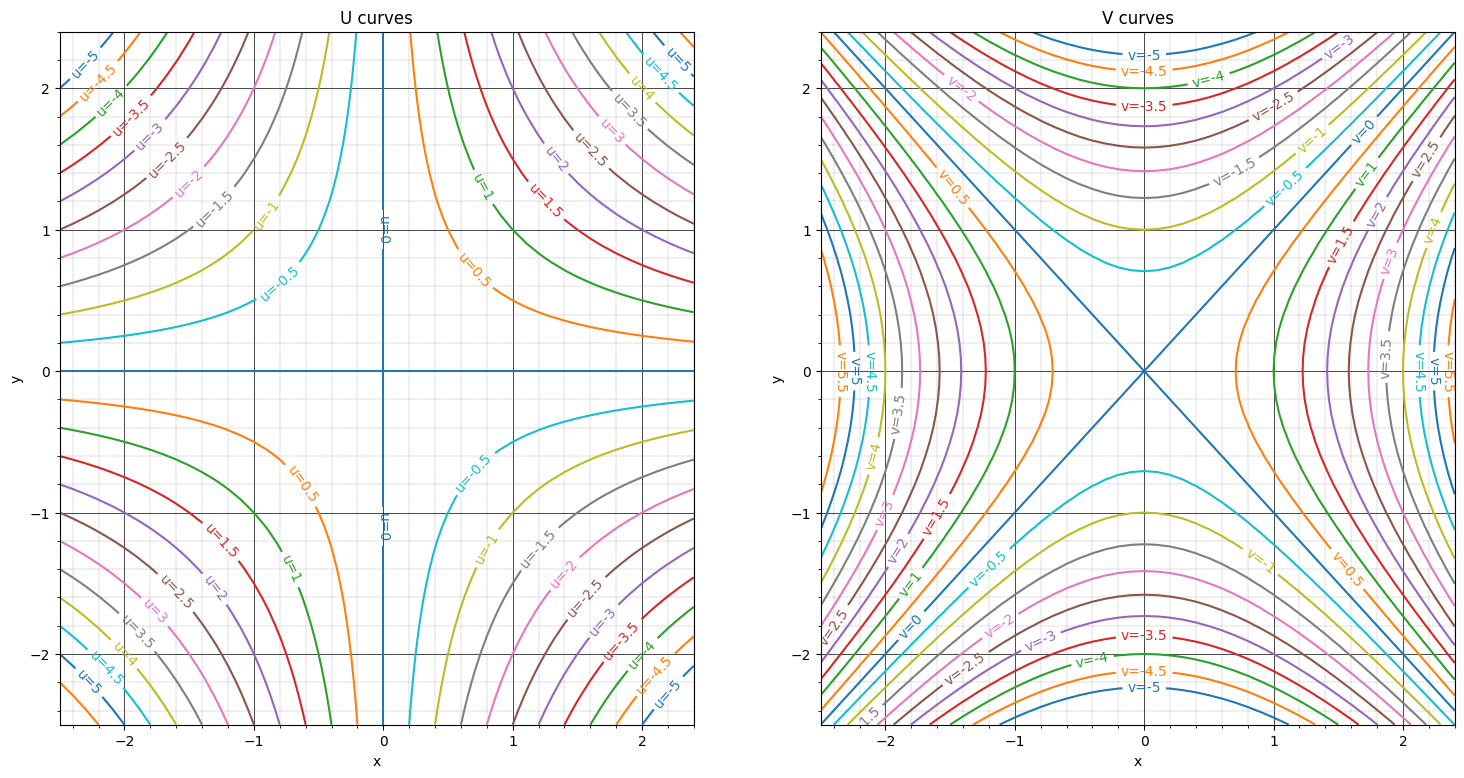
\includegraphics[width=\linewidth]{Q1B.png}
    \caption{U and V curves.}
    \label{fig:Q1B}
\end{figure}

\begin{figure}[H]
    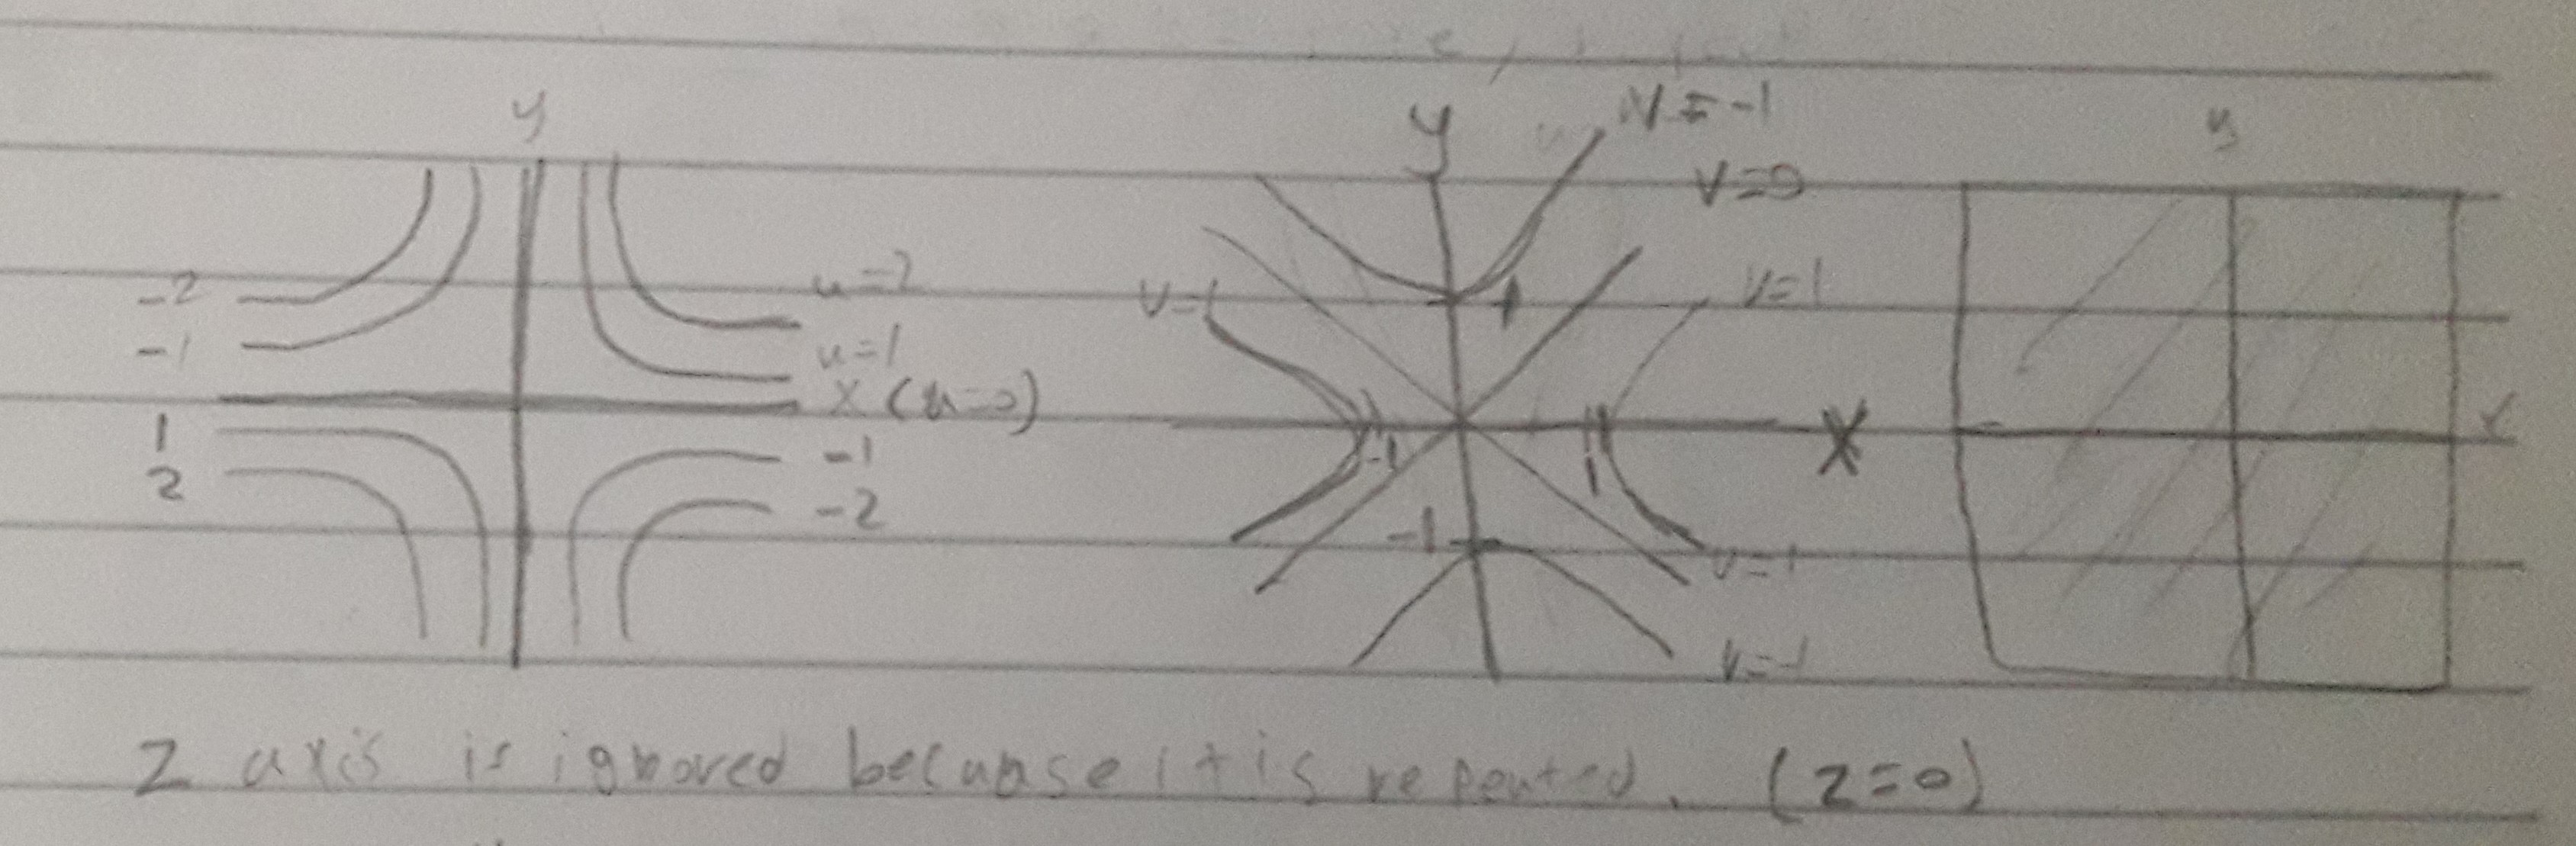
\includegraphics[width=\linewidth]{Q1B.jpg}
    \caption{U and V curves sketch.}
    \label{fig:Q1B2}
\end{figure}

\subsection{c}

\[
    \nabla u = \frac{ \partial u}{\partial x} \hat{\dot{\imath}} + \frac{ \partial u}{\partial y}  \hat{\dot{\jmath}} = \frac{ \partial (xy)}{\partial x}  \hat{\dot{\imath}} + \frac{ \partial (xy)}{\partial y}  \hat{\dot{\jmath}} = y  \hat{\dot{\imath}} + x  \hat{\dot{\jmath}}
\]

\[
    \nabla v = \frac{ \partial v}{\partial x} \hat{\dot{\imath}} + \frac{ \partial v}{\partial y}  \hat{\dot{\jmath}} = \frac{ \partial (x^2 - y^2)}{\partial x}  \hat{\dot{\imath}} + \frac{ \partial (x^2 - y^2)}{\partial y}  \hat{\dot{\jmath}} = 2x  \hat{\dot{\imath}} - 2y  \hat{\dot{\jmath}}
\]

\[
    \hat{e}_u = \frac{\nabla u}{|\nabla u|} = \frac{y  \hat{\dot{\imath}} + x  \hat{\dot{\jmath}}}{\sqrt{x^2 + y^2}}
\]

\[
    \hat{e}_v = \frac{\nabla v}{|\nabla v|} = \frac{2x  \hat{\dot{\imath}} - 2y  \hat{\dot{\jmath}}}{\sqrt{4x^2 + 4y^2}}
\]

\begin{figure}[H]
    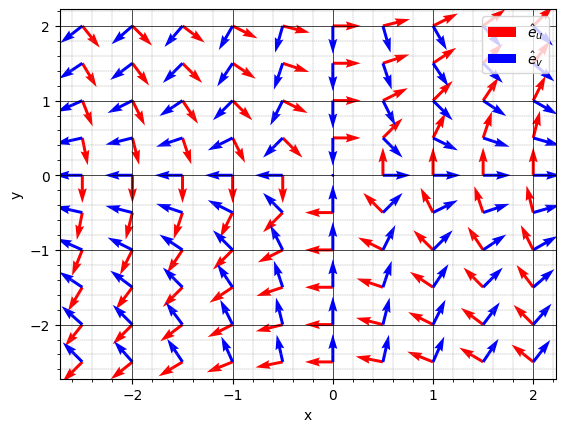
\includegraphics[width=\linewidth]{Q1C.png}
    \caption{Basis Vectors Field Plot}
    \label{fig:Q1C}
\end{figure}

\begin{figure}[H]
    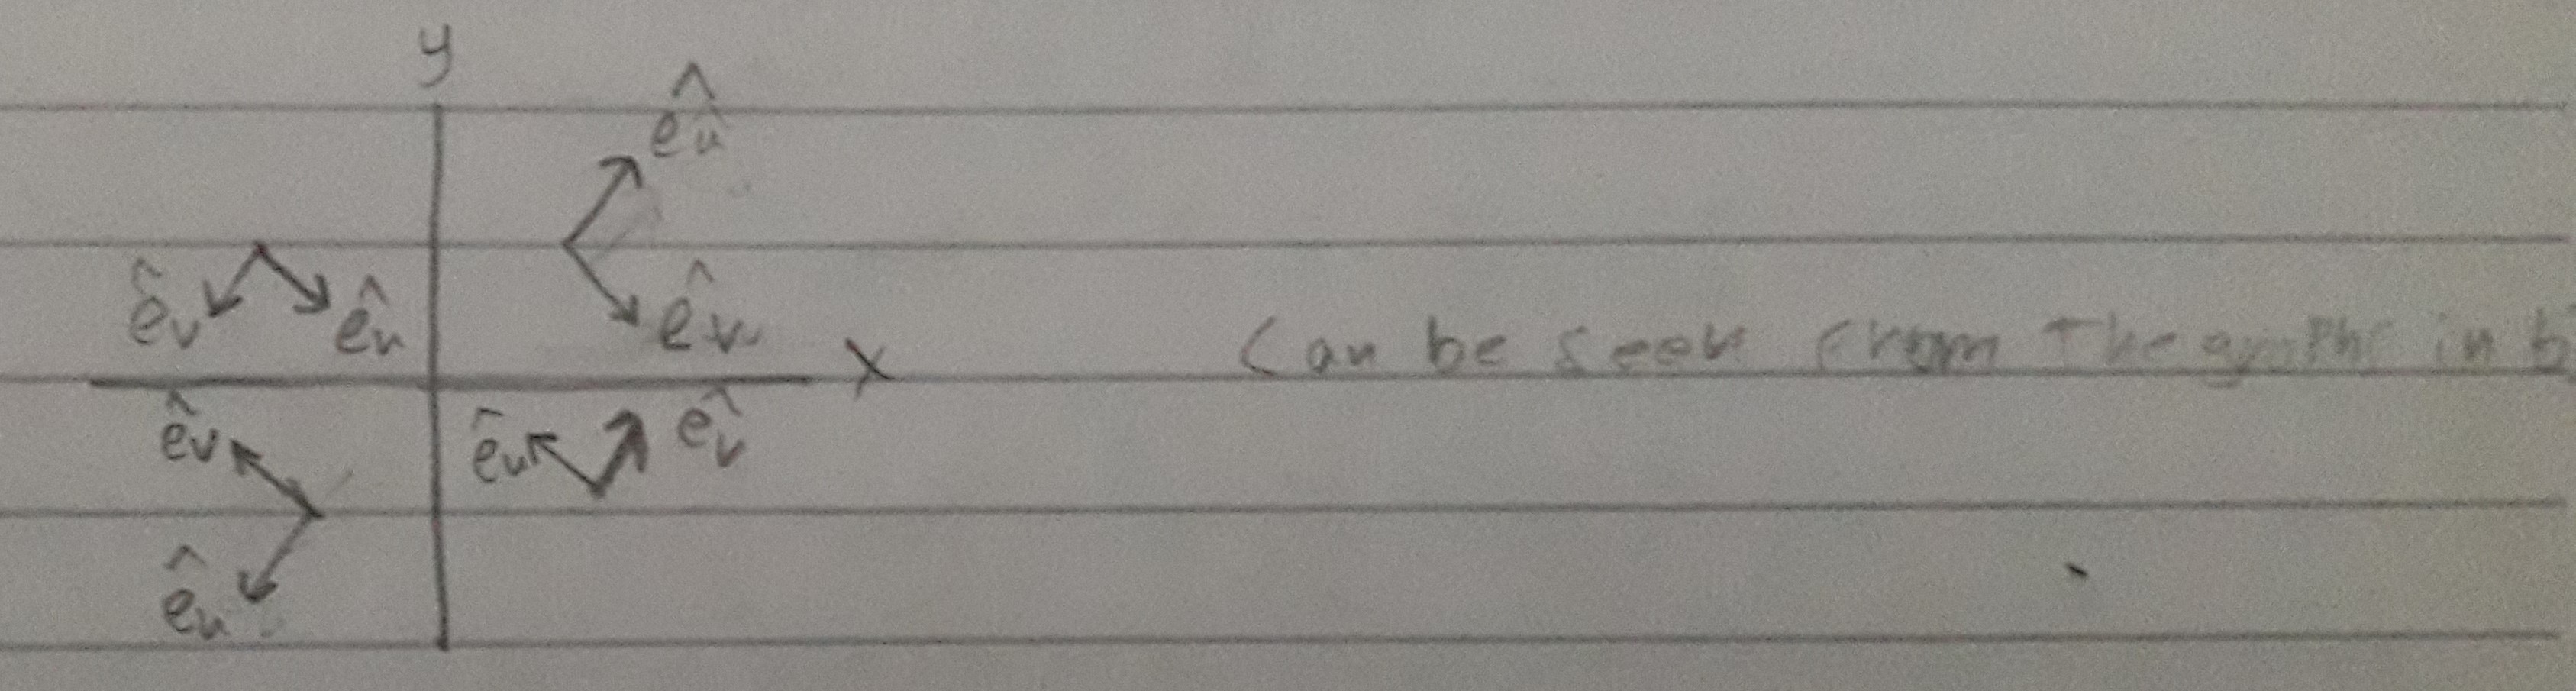
\includegraphics[width=\linewidth]{Q1C.jpg}
    \caption{Basis Vectors Field Plot sketch.}
    \label{fig:Q1C2}
\end{figure}

\subsection{d}

\[
    \hat{e}_u \times \hat{e}_v =
    \begin{vmatrix}
        \hat{\dot{\imath}}         & \hat{\dot{\jmath}}          & \hat{k} \\
        \frac{y}{\sqrt{x^2 + y^2}} & \frac{x}{\sqrt{x^2 + y^2}}  & 0       \\
        \frac{x}{\sqrt{x^2 + y^2}} & -\frac{y}{\sqrt{x^2 + y^2}} & 0       \\
    \end{vmatrix}
\]

\[
    = \left( - \frac{y}{\sqrt{x^2 + y^2}} \frac{y}{\sqrt{x^2 + y^2}} - \frac{x}{\sqrt{x^2 + y^2}} \frac{x}{\sqrt{x^2 + y^2}} \right)\hat{k} = -\hat{k}
\]

From the previous result, we can see that the coordinate system is left-handed.

\section{3.10.4}

\(\hat{e}_1\) is the unit vector in the direction of increasing \(q_1\).

\(\hat{e}_1 = \left\langle1, 0, 0\right\rangle \)

\subsection{a}

\[
    \nabla \cdot \textbf{V} = \frac{1}{h_1 h_2 h_3}\left[\frac{\partial}{\partial q_1}\left(V_1 h_2 h_3\right) + \frac{\partial}{\partial q_2}\left(V_2 h_1 h_3\right) + \frac{\partial}{\partial q_3}\left(V_3 h_1 h_2\right)\right]
\]

\[
    \nabla \cdot \hat{e}_1 = \frac{1}{h_1 h_2 h_3}\left[\frac{\partial}{\partial q_1}\left(1 * h_2 h_3\right) + \frac{\partial}{\partial q_2}\left(0 * h_1 h_3\right) + \frac{\partial}{\partial q_3}\left(0 * h_1 h_2\right)\right]
\]

\[
    \nabla \cdot \hat{e}_1 = \frac{1}{h_1 h_2 h_3} \frac{\partial}{\partial q_1}\left(h_2 h_3\right)
\]

\subsection{b}

\[
    \nabla \times \textbf{V} = \frac{1}{h_1 h_2 h_3}
    \begin{vmatrix}
        \hat{e}_1 h_1                 & \hat{e}_2 h_2                 & \hat{e}_3 h_3                 \\
        \frac{\partial}{\partial q_1} & \frac{\partial}{\partial q_2} & \frac{\partial}{\partial q_3} \\
        h_1 V_1                       & h_2 V_2                       & h_3 V_3                       \\
    \end{vmatrix}
\]

\[
    \nabla \times \hat{e}_1 = \frac{1}{h_1 h_2 h_3}
    \begin{vmatrix}
        \hat{e}_1 h_1                 & \hat{e}_2 h_2                 & \hat{e}_3 h_3                 \\
        \frac{\partial}{\partial q_1} & \frac{\partial}{\partial q_2} & \frac{\partial}{\partial q_3} \\
        h_1*1                         & h_2*0                         & h_3*0                         \\
    \end{vmatrix}
\]

\[
    \nabla \times \hat{e}_1 = \frac{1}{h_1 h_2 h_3}\left(\hat{e}_2 h_2 \frac{\partial h_1}{\partial q_3} - \hat{e}_3 h_3 \frac{\partial h_1}{\partial q_2} \right)
\]

\[
    \nabla \times \hat{e}_1 = \frac{1}{h_1}\left[\hat{e}_2 \frac{1}{h_3} \frac{\partial h_1}{\partial q_3} - \hat{e}_3  \frac{1}{h_2}  \frac{\partial h_1}{\partial q_2} \right]
\]

\section{3.10.5}

\section{3.10.28}

\section{3.10.29}

\section{3.10.30}

\subsection{a}

\subsection{b}

\section{3.10.31}

\section{3.10.32}

\subsection{a}

\subsection{b}

\subsection{c}

\end{document}